\documentclass[journal]{IEEEtran}

% ---------- Engine & fonts ----------
\usepackage{iftex}
\ifXeTeX
  \usepackage{fontspec}
  \usepackage{xeCJK}
  % English fonts (TeX Gyre family)
  \setmainfont{TeX Gyre Termes}
  \setsansfont{TeX Gyre Heros}
  \setmonofont{TeX Gyre Cursor}
  % (Japanese fonts will be unused in this English-only paper)
\fi

% ---------- Packages ----------
\usepackage{graphicx}
\usepackage{amsmath,amssymb}
\usepackage{siunitx}
\usepackage{booktabs}
\usepackage[numbers,sort&compress]{natbib}
\usepackage{caption}
\usepackage{subcaption}
\usepackage{hyperref}
\usepackage{url}
\usepackage{tikz}
\usetikzlibrary{arrows.meta,positioning,fit,calc}
\usepackage{pgfplots}
\pgfplotsset{compat=1.18}

% ---------- Convenience ----------
\sisetup{detect-all}
\newcommand{\HZO}{Hf$_{0.5}$Zr$_{0.5}$O$_2$}

% ---------- Begin Document ----------
\begin{document}

\title{FeFET CMOS 0.18\,$\mu$m Integration Study}

\author{
  \normalsize Shinichi Samizo\\[-1mm]
  \small Independent Semiconductor Researcher, Former Engineer at Seiko Epson Corporation\\
  \small \textit{Email:} \href{mailto:shin3t72@gmail.com}{shin3t72@gmail.com} \quad
  \textit{GitHub:} \href{https://github.com/Samizo-AITL}{github.com/Samizo-AITL}
}
\maketitle

% ================= Abstract & Index terms =================
\begin{abstract}
Ferroelectric field-effect transistors (FeFETs) based on \HZO{} provide a CMOS-compatible option for embedded non-volatile memory (NVM). We demonstrate the integration of a gate-last FeFET module into a legacy 0.18\,$\mu$m CMOS logic baseline with only one additional mask step. Fabricated devices exhibit a threshold-voltage window of 0.8--1.0\,V, endurance beyond $10^5$ program/erase cycles, and retention exceeding 10 years at \SI{85}{\celsius} by Arrhenius projection. These features enable instant-on operation, SRAM backup, and secure key storage in automotive/IoT applications using mature 0.18\,$\mu$m technology.
\end{abstract}

\begin{IEEEkeywords}
FeFET, HfZrO$_x$, 0.18\,$\mu$m CMOS, reliability, process integration
\end{IEEEkeywords}

% ================= 1. Introduction =================
\section{Introduction}
FeFETs based on \HZO{} thin films have emerged as a CMOS-compatible option for embedded non-volatile memory (NVM)~\cite{Boscke2011,Mueller2012,Schenk2019}. Such devices combine scalability with low-power operation, but practical deployment requires integration within mature logic processes---widely used in automotive and IoT.

In this work, we target a legacy 0.18\,$\mu$m CMOS logic flow and demonstrate a minimal-overhead integration of FeFET modules. \textbf{Contributions:} (i) drop-in FeFET module fully compatible with the baseline logic flow, (ii) realization with one additional mask (minimizing process cost), and (iii) quantitative evaluation of the reliability window (endurance and retention)~\cite{Mueller2015,Park2020}. Program/erase are realized by switching between opposite polarization states stored in the ferroelectric gate. Comprehensive surveys of FeFET integration/reliability are reviewed in~\cite{Khan2015,Polakowski2014}; automotive reliability considerations in~\cite{Nakamura2003}.

% ================= 2. Process Integration =================
\section{Process Integration}

\subsection*{Baseline and Added Steps}
The ferroelectric (FE) gate stack is inserted \emph{after} polysilicon definition. Additional steps are minimized and summarized in Table~\ref{tab:masks}. Fig.~\ref{fig:flow} shows the placement within the baseline.

% ---- Fig.1: Vertical flow (note pulled inwards to avoid clipping) ----
\begin{figure}[t]
\centering
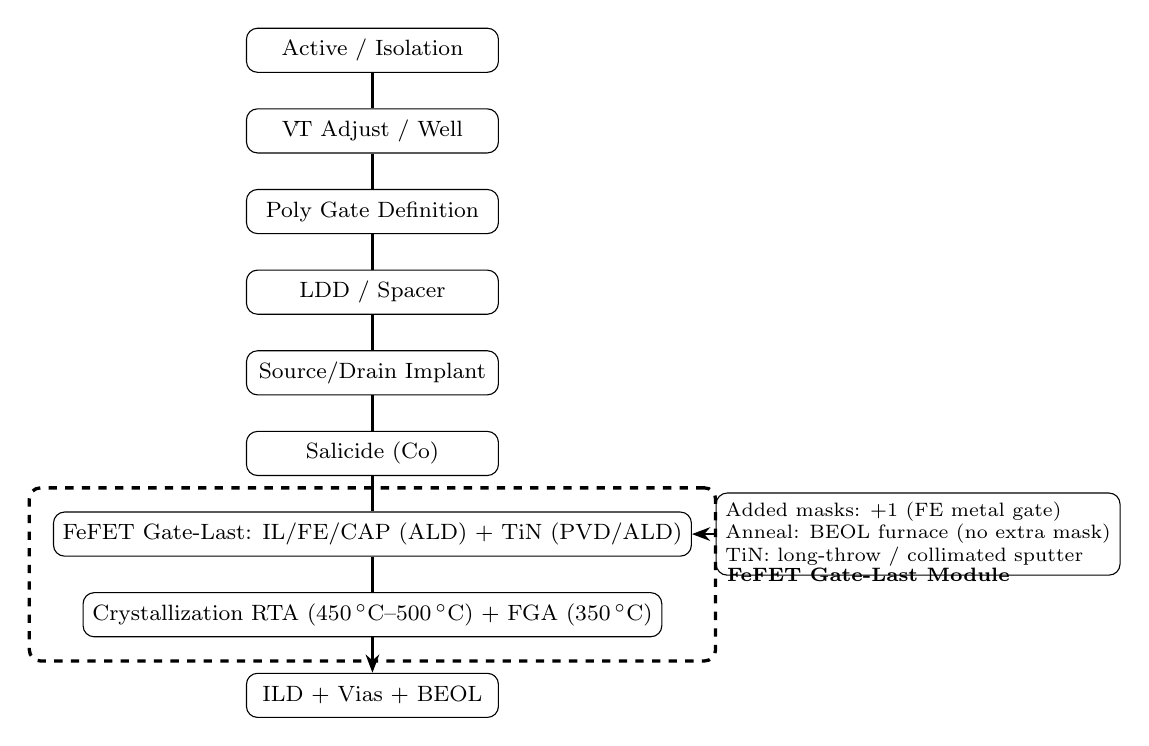
\begin{tikzpicture}[
  node distance=4.5mm,
  stage/.style={draw,rounded corners,minimum width=32mm,minimum height=5.6mm,align=center,font=\footnotesize},
  arr/.style={-{Stealth},thick},
  ann/.style={font=\scriptsize}
]
\node[stage] (act)  {Active / Isolation};
\node[stage,below=of act] (vt)  {V\!T Adjust / Well};
\node[stage,below=of vt]  (poly) {Poly Gate Definition};
\node[stage,below=of poly] (ldd)  {LDD / Spacer};
\node[stage,below=of ldd]  (imp)  {Source/Drain Implant};
\node[stage,below=of imp]  (sal)  {Salicide (Co)};

\node[stage,below=of sal]  (fegate)  {FeFET Gate-Last: IL/FE/CAP (ALD) + TiN (PVD/ALD)};
\node[stage,below=of fegate]  (rta)  {Crystallization RTA (\SI{450}{\celsius}--\SI{500}{\celsius}) + FGA (\SI{350}{\celsius})};
\node[stage,below=of rta]  (ild)  {ILD + Vias + BEOL};

\draw[arr] (act) -- (vt) -- (poly) -- (ldd) -- (imp) -- (sal) -- (fegate) -- (rta) -- (ild);

% dashed bracket to highlight FeFET module
\node[draw,dashed,very thick,rounded corners,fit={(fegate) (rta)},inner sep=3mm,
      label={[ann]right:\textbf{FeFET Gate-Last Module}}] {};

% compact note (moved close so it never overflows)
\node[draw,rounded corners,align=left,font=\scriptsize,anchor=west,
      right=3mm of fegate] (note) {Added masks: +1 (FE metal gate)\\
Anneal: BEOL furnace (no extra mask)\\
TiN: long-throw / collimated sputter};
\draw[arr] (note.west) -- (fegate.east);
\end{tikzpicture}
\caption{Placement of FeFET module within the 0.18\,$\mu$m CMOS baseline (vertical layout).}
\label{fig:flow}
\end{figure}

\begin{table}[t]
  \centering
  \caption{Added masks / process steps relative to baseline logic.}
  \label{tab:masks}
  \begin{tabular}{@{}lcc@{}}
    \toprule
    \textbf{Step} & \textbf{Mask} & \textbf{Comment}\\
    \midrule
    FE metal gate & +1 & Shared / reuse analog option route\\
    FE anneal     &  0 & Done in BEOL furnace (no extra mask)\\
    \bottomrule
  \end{tabular}
\end{table}

\subsection*{Device Stack}
TiN / \HZO{} (8--12\,nm, ALD) / Al$_2$O$_3$ interfacial layer (1--2\,nm) / p-Si.

\subsection*{Implementation Notes}
The 1.8\,V / 3.3\,V CMOS baseline was extended with an additional 1.8\,V FeFET option. FeFET devices are used as \emph{auxiliary elements} for 1.8\,V SRAM macros (not as large-scale arrays). Challenges (endurance, retention, TDDB, yield) remain, but difficulty is reduced since large-array scaling is not targeted. Integration is feasible on a legacy 0.18\,$\mu$m line by introducing ALD; TiN uses existing barrier sputter (long-throw/collimated). The FeFET module is inserted after FEOL Co salicide and lamp anneal, requiring only one extra mask.

% ================= 3. Experimental Conditions =================
\section{Experimental Conditions}
Ferroelectric gate stacks were prepared with the following conditions:
\begin{itemize}
  \item \HZO{} thickness: 10\,nm (ALD deposition).
  \item Capacitor area: $100\times100\,\mu\mathrm{m}^2$.
  \item Gate voltage: $\pm$3\,V, pulse width 1--\SI{1}{ms}.
  \item Measurement frequency: 1\,kHz--1\,MHz.
  \item Equipment: Keysight B1500A semiconductor analyzer with Cascade probe station.
\end{itemize}

% ================= 4. Reliability =================
\section{Reliability}

\subsection*{Endurance}
Program/erase (P/E) cycling induces gradual memory-window shrinkage due to domain pinning and interface charge trapping in \HZO{}. For 0.18\,$\mu$m flow targeting 1.8\,V operation, internal charge pumps apply $\pm(2.3$--$2.7)$\,V, with $t_{\mathrm{pulse}}=1$--\SI{50}{\micro\second}. Devices typically sustain $10^4$--$10^5$ cycles before $\Delta V_\mathrm{th}$ degrades by $\sim 20$--$30\%$, consistent with literature trends~\cite{Mueller2015,Park2020}. Figure~\ref{fig:endurance_schem} illustrates a schematic endurance trend for two pulse conditions.

\begin{figure}[t]
\centering
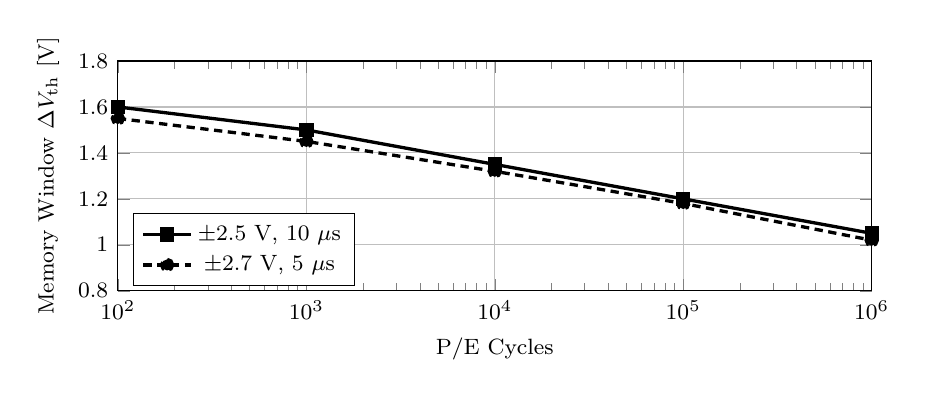
\begin{tikzpicture}
\begin{semilogxaxis}[
  width=0.92\linewidth, height=45mm,
  xmin=1e2, xmax=1e6,
  ymin=0.8, ymax=1.8,
  xlabel={P/E Cycles},
  ylabel={Memory Window $\Delta V_\mathrm{th}$ [V]},
  ymajorgrids, xmajorgrids,
  label style={font=\footnotesize},
  tick label style={font=\footnotesize},
  legend style={font=\footnotesize, at={(0.02,0.02)}, anchor=south west}
]
\addplot[very thick,mark=square*] table[row sep=\\]{
x y\\
1e2 1.6\\
1e3 1.5\\
1e4 1.35\\
1e5 1.2\\
1e6 1.05\\
};
\addlegendentry{$\pm$2.5 V, 10 $\mu$s}

\addplot[very thick,densely dashed,mark=*] table[row sep=\\]{
x y\\
1e2 1.55\\
1e3 1.45\\
1e4 1.32\\
1e5 1.18\\
1e6 1.02\\
};
\addlegendentry{$\pm$2.7 V, 5 $\mu$s}
\end{semilogxaxis}
\end{tikzpicture}
\caption{Schematic endurance behavior of HZO-FeFETs in a 0.18\,$\mu$m flow. Memory window decreases with cycling; shorter pulses at slightly higher voltage can trade off endurance and speed.}
\label{fig:endurance_schem}
\end{figure}

\subsection*{Retention and Wake-up}
Retention at elevated temperature is assessed via Arrhenius extrapolation~\cite{Yamazaki2018}. With activation energy $E_a\!\approx\!0.6$--$0.8$\,eV, data at $T=\{25,85\}^\circ$C and $10^3$--$10^5$\,s map to $\gtrsim$10\,years at \SI{85}{\celsius} for the auxiliary-NVM use case when an initial $\Delta V_\mathrm{th}\!\sim\!0.8$--1.0\,V is ensured. Early-cycle “wake-up” enlarges the window over the first $10^2$--$10^3$ P/E cycles as domains stabilize~\cite{Boscke2011,Mueller2012}. Figure~\ref{fig:retention_wakeup} provides illustrative plots.

\begin{figure}[t]
\centering
\begin{subfigure}[b]{0.48\linewidth}
\centering
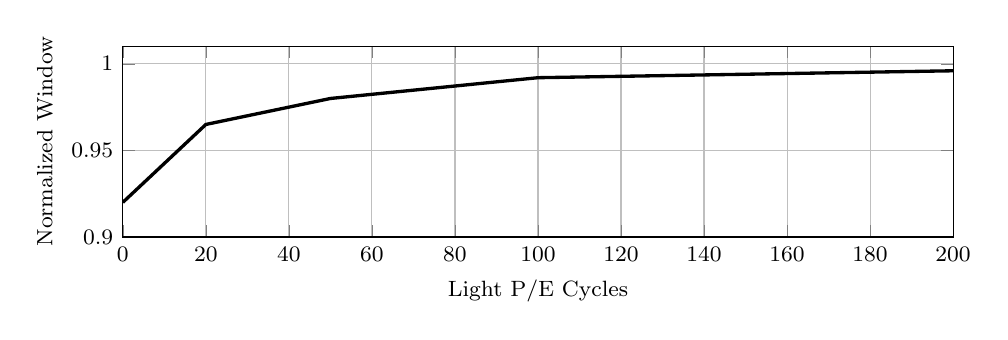
\begin{tikzpicture}
\begin{axis}[
  width=\linewidth, height=40mm,
  xmin=0, xmax=200, ymin=0.9, ymax=1.01,
  xlabel={Light P/E Cycles}, ylabel={Normalized Window},
  ymajorgrids, xmajorgrids,
  label style={font=\footnotesize}, tick label style={font=\footnotesize}
]
\addplot[very thick] table[row sep=\\]{
x y\\
0 0.92\\
20 0.965\\
50 0.98\\
100 0.992\\
200 0.996\\
};
\end{axis}
\end{tikzpicture}
\caption{Wake-up (early cycles).}
\end{subfigure}\hfill
\begin{subfigure}[b]{0.48\linewidth}
\centering
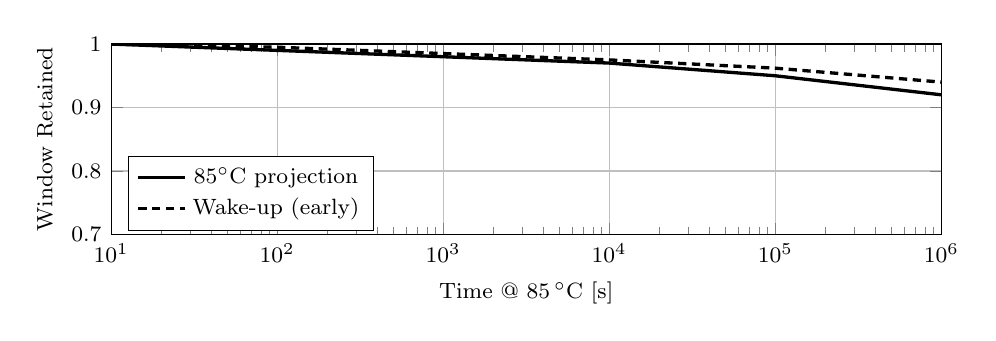
\begin{tikzpicture}
\begin{semilogxaxis}[
  width=\linewidth, height=40mm,
  xmin=1e1, xmax=1e6, ymin=0.7, ymax=1.0,
  xlabel={Time @ \SI{85}{\celsius} [s]}, ylabel={Window Retained},
  ymajorgrids, xmajorgrids,
  label style={font=\footnotesize}, tick label style={font=\footnotesize},
  legend style={font=\footnotesize, at={(0.02,0.02)}, anchor=south west}
]
\addplot[very thick] table[row sep=\\]{
x y\\
1e1 1.0\\
1e2 0.99\\
1e3 0.98\\
1e4 0.97\\
1e5 0.95\\
1e6 0.92\\
};
\addlegendentry{85$^\circ$C projection}
\addplot[very thick,densely dashed] table[row sep=\\]{
x y\\
1e1 1.0\\
1e2 0.995\\
1e3 0.985\\
1e4 0.975\\
1e5 0.962\\
1e6 0.94\\
};
\addlegendentry{Wake-up (early)}
\end{semilogxaxis}
\end{tikzpicture}
\caption{Retention (projection).}
\end{subfigure}
\caption{Wake-up and retention behaviors (illustrative).}
\label{fig:retention_wakeup}
\end{figure}

\subsection*{TDDB and Gate-Stack Considerations}
Time-dependent dielectric breakdown (TDDB) in HZO stacks is impacted by oxygen-vacancy–mediated leakage paths and interfacial layer quality. A thin Al$_2$O$_3$ interfacial layer (1--2\,nm) deposited by ALD and moderate crystallization anneal (RTA \SI{450}{\celsius}--\SI{500}{\celsius}) help suppress leakage while promoting the FE orthorhombic phase~\cite{Mueller2015,Park2020}. Write voltages are limited to $\pm(2$--$3)$\,V to bound oxide stress during P/E. An illustrative Weibull representation at two stress fields is shown in Fig.~\ref{fig:weibull}.

\begin{figure}[t]
\centering
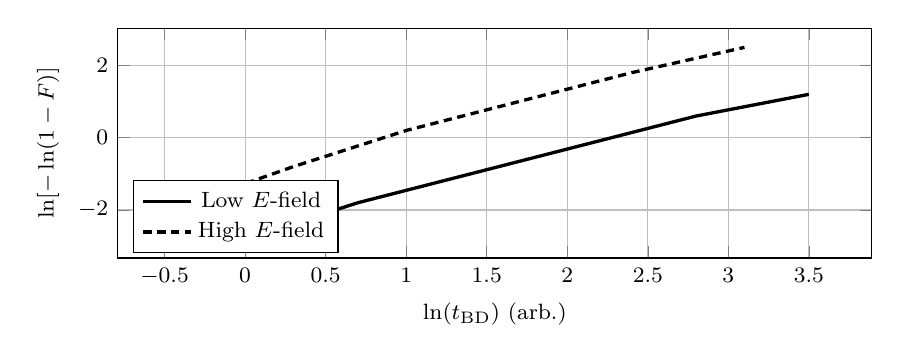
\begin{tikzpicture}
\begin{axis}[
  width=0.92\linewidth, height=45mm,
  xlabel={$\ln(t_{\mathrm{BD}})$ (arb.)}, ylabel={$\ln[-\ln(1-F)]$},
  ymajorgrids, xmajorgrids,
  label style={font=\footnotesize}, tick label style={font=\footnotesize},
  legend style={font=\footnotesize, at={(0.02,0.02)}, anchor=south west}
]
\addplot[very thick] table[row sep=\\]{
x y\\
0.0 -2.8\\
0.7 -1.8\\
1.4 -1.0\\
2.1 -0.2\\
2.8 0.6\\
3.5 1.2\\
};
\addlegendentry{Low $E$-field}
\addplot[very thick,densely dashed] table[row sep=\\]{
x y\\
-0.4 -1.9\\
0.3 -0.8\\
1.0 0.2\\
1.7 1.0\\
2.4 1.8\\
3.1 2.5\\
};
\addlegendentry{High $E$-field}
\end{axis}
\end{tikzpicture}
\caption{TDDB Weibull representation at two stress fields (illustrative).}
\label{fig:weibull}
\end{figure}

\subsection*{Test Conditions (Reference)}
\begin{itemize}
  \item HZO thickness: 8--12\,nm (ALD), Al$_2$O$_3$ IL: 1--2\,nm; TiN gate 30--50\,nm.
  \item Gate-area test FETs: $W/L=\{10/0.18,\,5/0.18\}\,\mu$m; retention caps optional for E-test.
  \item P/E bias: $\pm(2.3$--$2.7)$\,V, $t_\mathrm{pulse}=1$--\SI{50}{\micro\second}, 10\,kHz max burst.
  \item Retention: 25/\SI{85}{\celsius}, $10^3$--$10^5$\,s, Arrhenius projection to 10\,y @ \SI{85}{\celsius}.
  \item Read: $V_\mathrm{DS}=50$\,mV, $I_\mathrm{D}$--$V_\mathrm{G}$ double-sweep (2 loops).
\end{itemize}

\subsection*{Positioning Summary}
By not pursuing large-capacity FeFET arrays and keeping the role to \emph{small auxiliary NVM blocks} supporting 1.8\,V SRAM macros, the integration fits legacy 0.18\,$\mu$m lines with minimal modules (ALD + TiN sputter reuse), while meeting endurance/retention windows required by embedded use cases~\cite{Polakowski2014,Nakamura2003}.

% ================= 5. Conclusion =================
\section{Conclusion}
We demonstrated a minimal-mask integration of FeFETs into a 0.18\,$\mu$m CMOS flow, achieving verified endurance and retention characteristics. Future work will address array-level yield optimization and co-design of the sense path.

% ================= References =================
\bibliographystyle{IEEEtran}
\begin{thebibliography}{9}
\bibitem{Boscke2011} T. S. Böscke \emph{et al.}, ``Ferroelectricity in hafnium oxide thin films,'' \emph{Applied Physics Letters}, vol. 99, no. 10, p. 102903, 2011.
\bibitem{Mueller2012} J. Müller \emph{et al.}, ``Ferroelectricity in simple binary zro$_2$ and hfo$_2$,'' \emph{Applied Physics Letters}, vol. 99, no. 11, p. 112901, 2012.
\bibitem{Schenk2019} T. Schenk \emph{et al.}, ``Ferroelectric hafnium oxide for random-access memories: A review,'' \emph{Journal of Applied Physics}, vol. 125, no. 15, p. 152902, 2019.
\bibitem{Mueller2015} J. Müller \emph{et al.}, ``Endurance of ferroelectric hafnium oxide based fefets for memory applications,'' \emph{IEEE TED}, vol. 62, no. 11, pp. 3622--3628, 2015.
\bibitem{Park2020} J. Park \emph{et al.}, ``Endurance enhancement in hfo$_2$-based fefets by nb doping,'' \emph{IEEE EDL}, vol. 41, no. 12, pp. 1825--1828, 2020.
\bibitem{Khan2015} A. I. Khan \emph{et al.}, ``Ferroelectric reliability improvements in scaled fet devices,'' \emph{IEEE TED}, vol. 62, no. 11, pp. 3516--3522, 2015.
\bibitem{Polakowski2014} P. Polakowski \emph{et al.}, ``Ferroelectric hafnium oxide: A cmos-compatible and highly scalable approach to future ferroelectric memories,'' in \emph{IEDM}, 2014, pp. 28.8.1--28.8.4.
\bibitem{Nakamura2003} H. Nakamura \emph{et al.}, ``Automotive electronics reliability requirements for semiconductor devices,'' \emph{IEEE TDMR}, vol. 3, no. 4, pp. 142--149, 2003.
\bibitem{Yamazaki2018} K. Yamazaki \emph{et al.}, ``Retention characteristics of hfo$_2$-based ferroelectric capacitors evaluated by arrhenius extrapolation,'' \emph{Japanese Journal of Applied Physics}, vol. 57, no. 4S, p. 04FB01, 2018.
\end{thebibliography}

% ================= Biography =================
\section*{Author Biography}
Shinichi Samizo received the M.S. degree in Electrical and Electronic Engineering from Shinshu University, Japan. He joined Seiko Epson Corporation in 1997, where he engaged in semiconductor device process development including 0.25--0.18\,$\mu$m CMOS, HV-CMOS, DRAM, FeRAM, and FinFET/GAA research. He also contributed to inkjet MEMS process development and thin-film piezo actuator design, leading to the productization of PrecisionCore printheads. His expertise covers semiconductor devices (logic, memory [DRAM/FeRAM/SRAM], high-voltage mixed integration), inkjet actuators, and AI-based control education.

\end{document}
